% Exempel på färdig-formaterad sång till VN:s
% sångbok 2010.

% Denna fil kan användas som sådan, bara verserna,
% namnen och annan rådata behöver bytas ur fälten.
% Tecknet "%" markerar en kommentar som helt och 
% hållet ignoreras av programmet som läser filen.

% Spara den färdiga filen som 
% 'SangnamnUtanMellanslagEllerSkander.tex'
% t.ex. blir "Vid En Källa" till 
% 'VidEnKalla.tex'
% Varje sång blir en egen fil.

\beginsong{Visa vid vindens ängar}[ 	% Börja sången här
	by={Mats Paulson},
	index={Det går en vind}]		% Alternativa
			% sångnamn
	
\beginverse*		% Börja vers
Det går en vind över vindens ängar,
det fladdrar till i en tyllgardin.
Och jag ska skriva en sommarvisa
med sol och blomdoft i melodin.
Jag ville sjunga om Katarina,
till träklangsflöjter och alcymbal
men vindens toner blir sommarns sånger,
jag bara lyssnar i björklövssal.
Det går en vind över vindens ängar,
det fladdrar till i en tyllgardin.
Och jag ska skriva en sommarvisa
med sol och blomdoft i melodin.
\endverse			% Sluta vers

\beginverse*		% Börja vers
Det går en flicka i aspelunden,
jag har ett gulnat fotografi.
Med åren blev hon en dröm, en saga,
en ensam vandrares sympati.
Jag ville skriva en liten visa
där ögonblick blir till evighet
men ord blir stumma och toner döda
och visans tanke blir hemlighet.
Det går en flicka i aspelunden,
jag har ett gulnat fotografi.
Med åren blev hon en dröm, en saga,
en ensam vandrares sympati.
\endverse			% Sluta vers
\endsong			% Sluta sång

\begin{figure}[!b]
\begin{center}
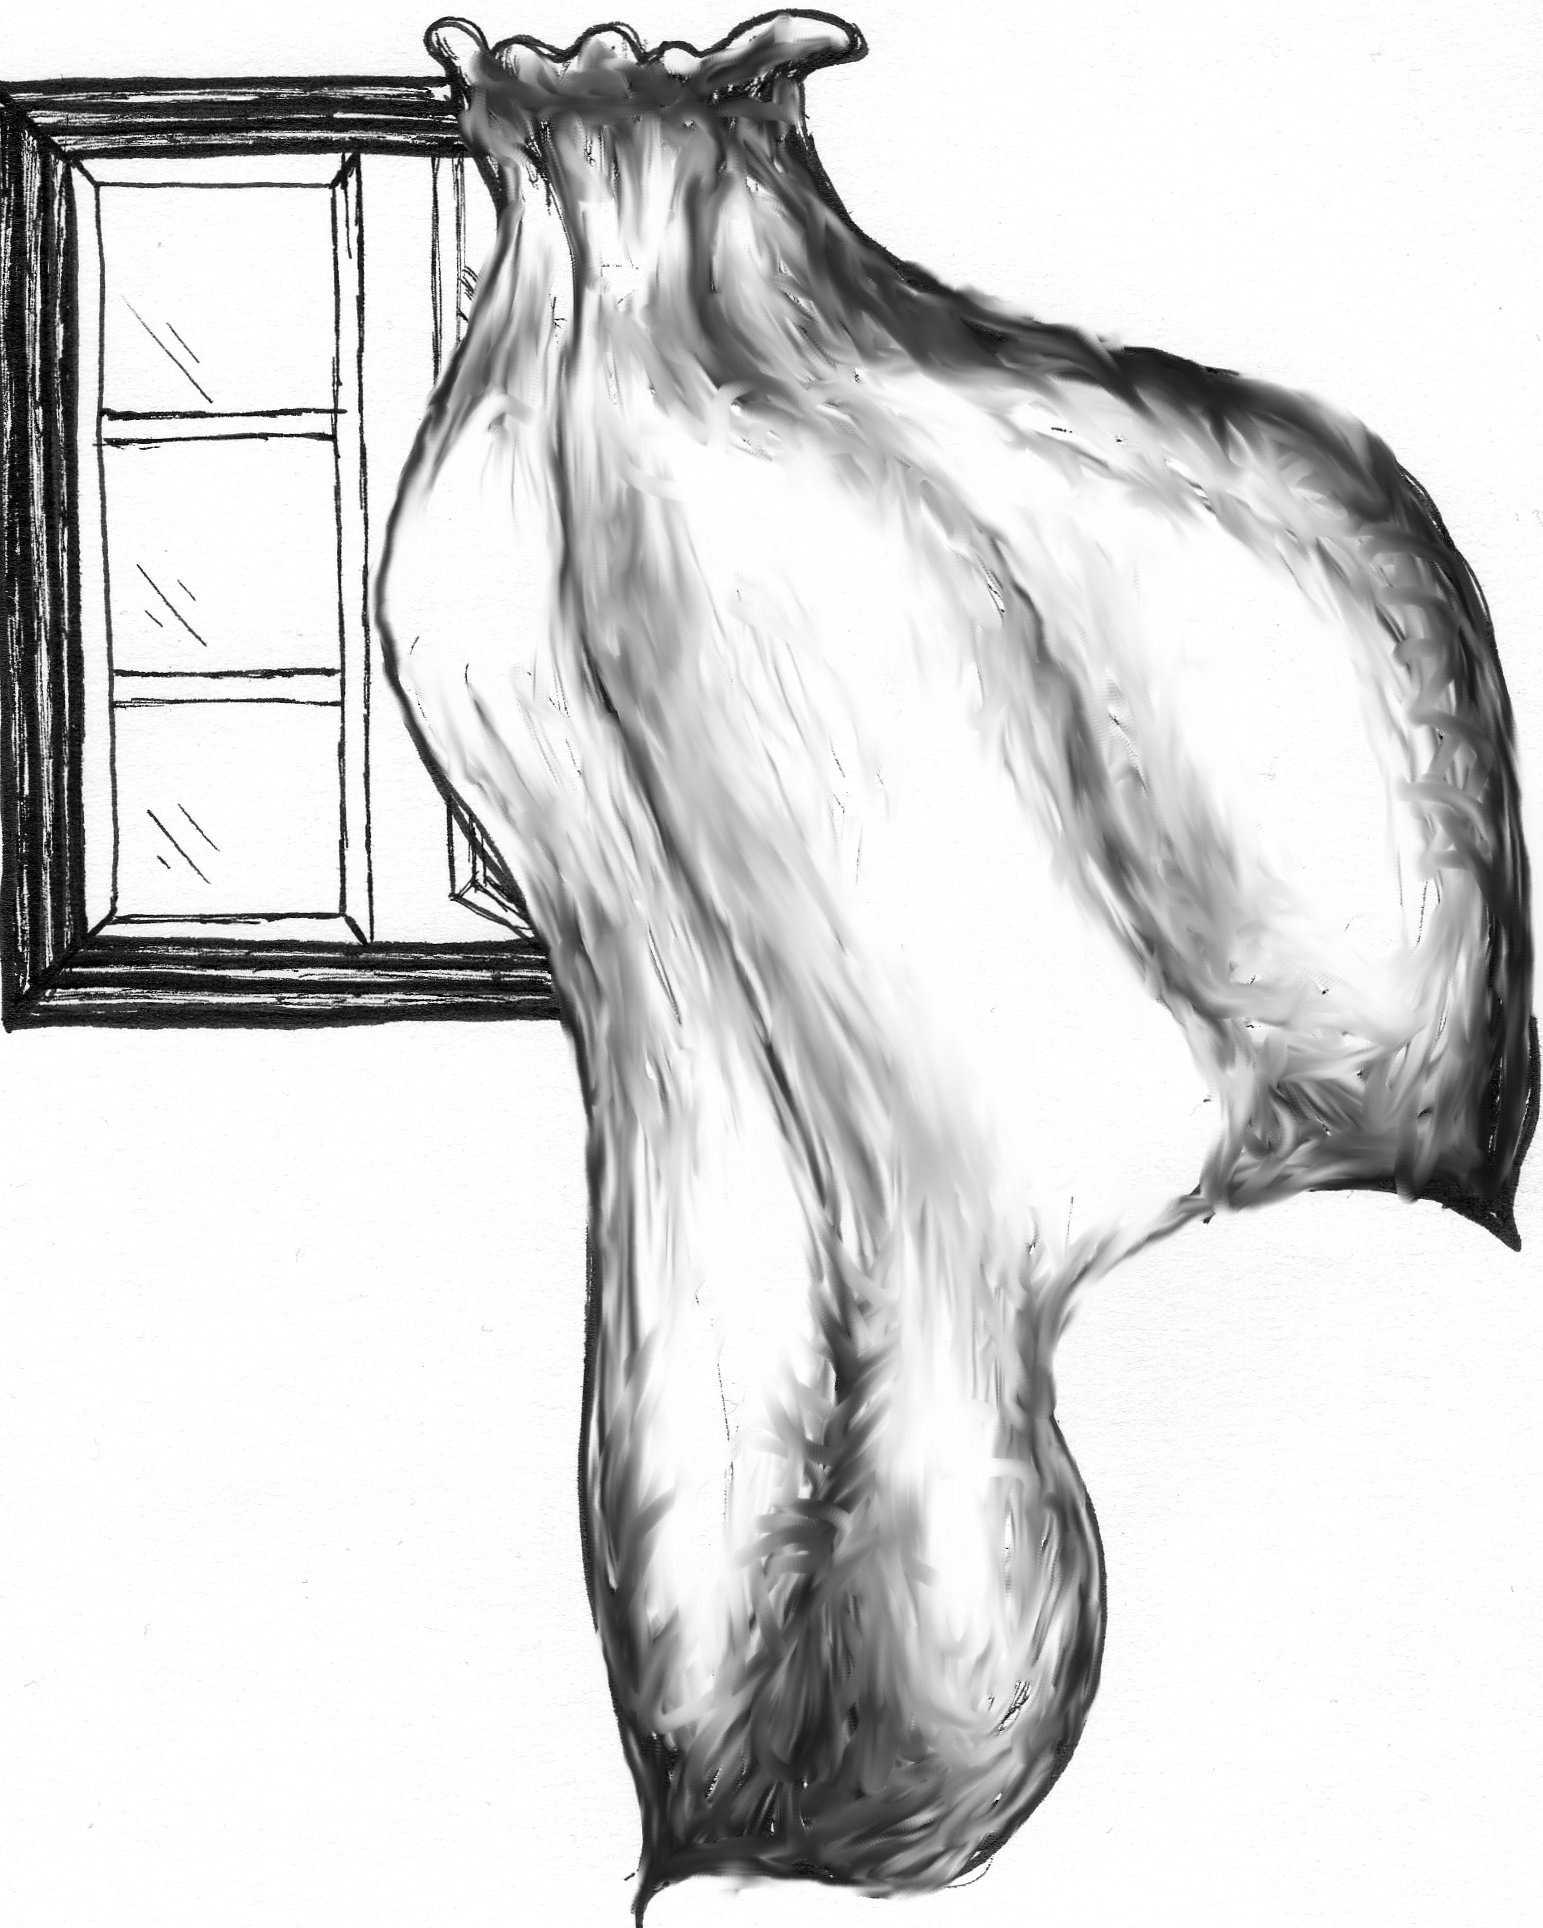
\includegraphics[scale=.4]{../bilder/tyllgardin.jpg} 
\end{center}
\end{figure}
